\section{Implementation}
As this was part of our access management platform we implemented this floorplan also in our web application.

\begin{figure}[!hb]
	\centering
	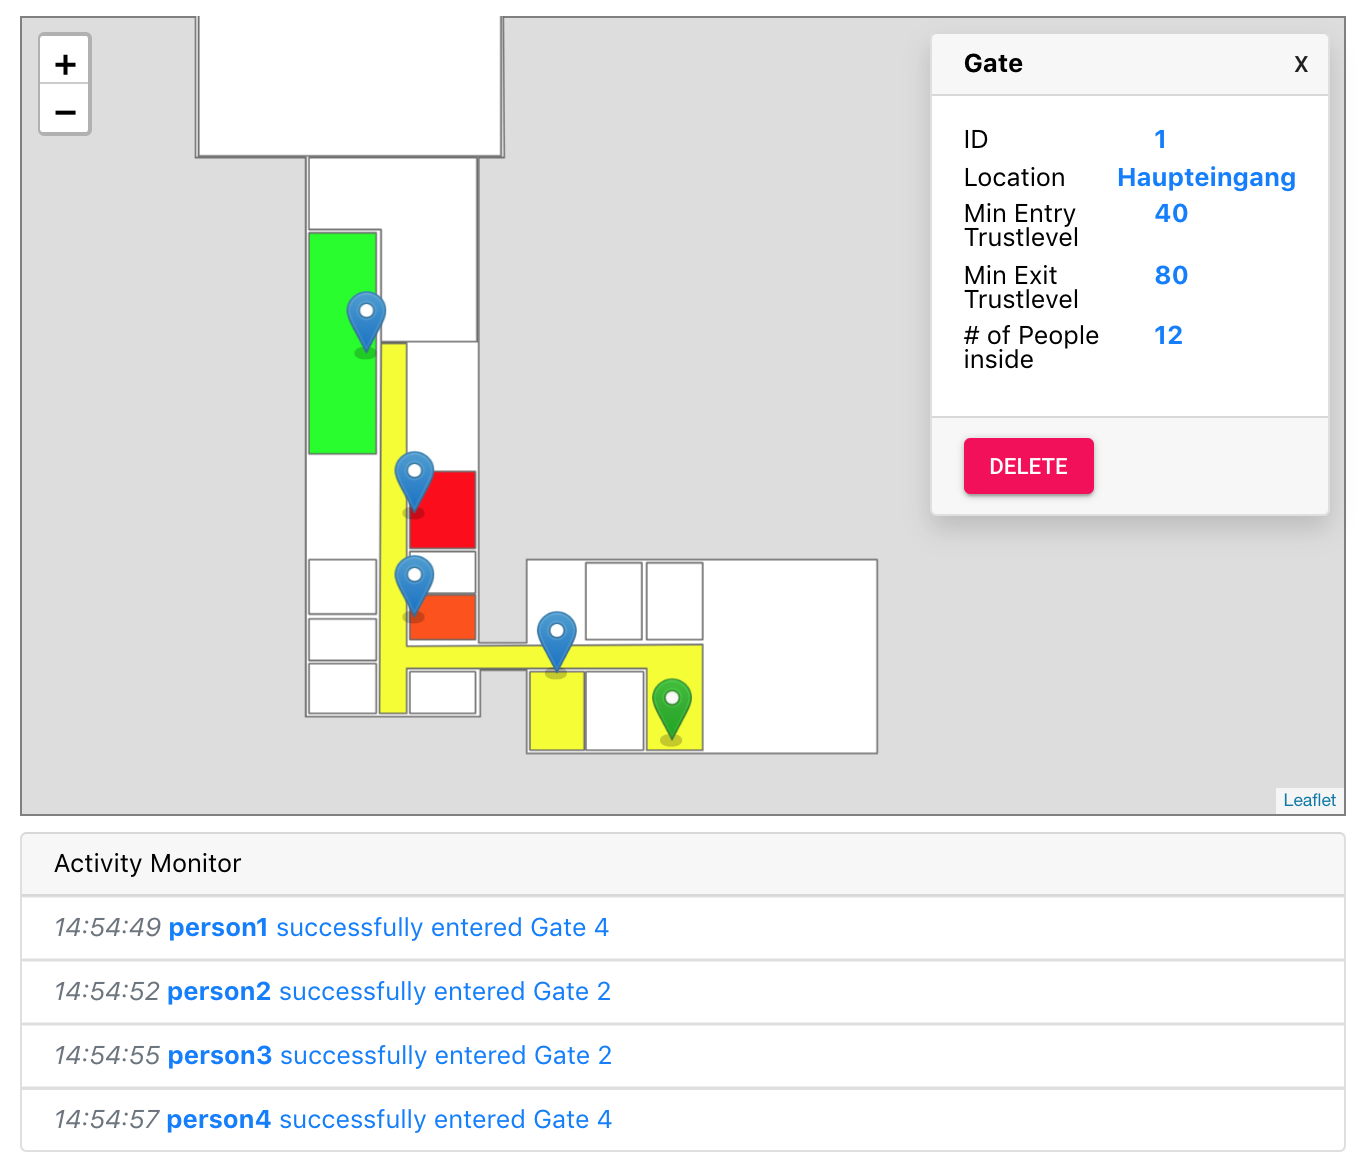
\includegraphics[width=0.9\linewidth]{images/FloorplanScreenshot}
	\caption{Screenshot of the implemented interactive floorplan}
	\label{fig:FloorplanScreenshot}
\end{figure}

\subsection{Display of indoor features}
\label{Display of indoor features}

\subsubsection{GeoJSON}
\label{GeoJSON}

GeoJSON is a format for interchanging geospatial data and is based on JavaScript Object Notation. With the publishing of RFC 7946 in August 2016 it has a standardized format specification.
Different Geometries can be represented in a GeoJSON file. These include for example Lines, Linestrings, Polygones or Multipolygones\footnote{\url{https://tools.ietf.org/html/rfc7946}}. 

This can be used to encode the geometry for countries, houses and streets on a map, but also for encoding data for indoor rooms, stairs and hallways.


\subsubsection{Leaflet}
\label{Leaflet}

Leaflet is another open-source JavaScript library for creating interactive maps. With it's first version released in 2011, it is a well established and tested library. 

By only including core features for map visualization, it only has a bundled size of 138.6KB\footnote{\url{https://bundlephobia.com/result?p=leaflet@1.5.1}}, making it a very lightweight library.

Furthermore Leaflet supports every browser and can easily be extended by plugins from the community.
This also includes plugins for creating indoor maps and real-time maps with Socket.IO. 

The indoor map plugin comes with support for loading in GeoJSON. We use the |L.Indoor| class to load in the geospatial data from a GeoJSON file:

\begin{lstlisting}[label=setupMap]
...
this.map = L.map('floorplan-container', {
            center: new L.LatLng(49.41873, 8.67689),
            zoom: 20,
        });

        const indoorLayer = new L.Indoor(this.props.geoJSON, {
        ...
\end{lstlisting}

This renders the geoJSON data on a map with a html layer for eachfeature.

\emph{TODO: latitude, longitude erklaeren}

%Considering the limited time we had for the implementation, we decided that Leaflet fits our needs the best and could be the fastest way to build our interactive live floorplan.


Hier erwaehnen das jedes feature eine ID benoetigt und so.

\subsection{Adding of markers}
\label{Adding of markers}

The floorplan handles mouse clicks on each room that is displayed. If a click event occurs, it adds a new marker at this position, which is then automatically linked with of the underlying room.

\begin{lstlisting}[label=addMarkers]
handleClickOnRoom = (event) => {
        this.addMarker(
          event.latlng, 
          { gateId: undefined, assignedRoomId: event.target.feature.id }, 
          true);
    };
\end{lstlisting}

To create this connection between the room and the marker, each feature/room in the GeoJSON file has to have a distinguashble member-attribute \emph{id}.

This is still following the GeoJSON format specification.

After setting the marker it needs to be linked with the gate. This is done via an Selection Input.



\subsection{Logging of Gate Events}
\label{Logging of Gate Events}

\subsubsection{Elastic Stack}
\label{Elastic Stack}

The Elastic Stack consists of mainly three open-source projects: \emph{Elasticsearch}, \emph{Logstash} and \emph{Kibana}.
Together they form a pipeline that can be used to analyze, search and visualize logs created from different sources. 

The component of the first stage of this pipeline is Logstash, which is responsible for collecting data from different locations and transforming it for the next step. Elasticsearch then indexes these logs and provides a RESTful API for searching. Kibana uses this API from Elasticsearch to provide meaningful visualization of the logs.
Through a smart indexing technology the Elastic Stack promises a fast response time even for large data sets and is used by companies like Netflix for monitoring security related logs or Medium for debugging production issues \footnote{\url{https://hackernoon.com/elastic-stack-a-brief-introduction-794bc7ff7d4f}}.

In our project logs sent from the gates need to be analyzed and visualized to give the FM Team more insights about the access decisions made. These informations get also displayed in the floorplan and the heatmap gets calculated based on the gate event logs. To ensure a fast display of the access decision data and to also ensure the possibility in the future to search and visualize logs not only from the gates, but from other sources also, we decided to include the Elastic Stack into our project.

Since were only working with events coming from one source, the gates, were not using Logstash. And since we provide own custom visualization Kibana is also not used.


Gates nutzen folgendes Endpunkt, ist abgesichert per pre shared token.



We only use the elasticsearch part. The elasticsearch exposes a RESTful API for searching.
We use this interface to count the exits and entries.
\begin{lstlisting}[label=searchElasticPOST]
function postGateEvent(eventData) {
    return fetch(`http://${elasticsearchBasePath}/gates/_doc`, {
        headers: {
            'Content-Type': 'application/json',
        },
        body: eventData,
        method: 'POST',
    })
        .then(response => errorHandling.checkResponseOk(response, msg.getCreateEventFailMsg(response)));
}
\end{lstlisting}

The gates have to transmit the ID of the device that tried to access, the access type (entry or exit), the gate ID, if the entry or exit was successful

\begin{lstlisting}[label=searchElasticGET]
function fetchAllEventsAtGateWithAccessType(gateId, accessType) {
    const now = new Date();
    const officeOpening = getOfficeOpeningDatetime();

    const url = `http://${elasticsearchBasePath}/gates/_search?sort=timestamp:desc&`
        + `q=gateId:${gateId}%20AND%20accessType=${accessType}%20AND%20timestamp:[${officeOpening.toISOString()}+TO+${now.toISOString()}}`;
    return fetch(url, {
        headers: {
            Accept: 'application/json',
        },
    })
        .then(response => errorHandling.checkResponseOk(response));
}
\end{lstlisting}


Hier sagen wie man herauskriegt wieviele da sind


Elasticstack routen, indexes bla


\subsection{Real-time Floorplan}
\label{Real-time Floorplan}

\subsubsection{Socket.IO}
\label{Socket.IO}

Socket.IO is a JavaScript library that makes it possible to implement real-time applications. This is achieved through an event-based, bidirectional communication between the client and the server. 

For this to work the client-side needs to install a Socket.IO javascript library and the server needs to run a Socket.IO Node server. 

Although Socket.IO also uses WebSockets for transportation it is not an implementation of the WebSocket-protocol. It extends and combines multiple real-time protocols and switches between them if needed. Therefore a connection can only be established between a Socket.IO client and a Socket.IO server\footnote{\url{https://socket.io/docs/index.html}}.

The frontend has to install and set the Socket.IO client and then listens for the events emitted from the backend.

\begin{lstlisting}[label=socketIOClientSide]
listenForGateEvents = () => {
        const socket = io({
            secure: true,
            transport: ['websocket'],
            query: {
                token: sessionStorage.getItem('kctoken'),
            },
            jsonp: false,
        });

        socket.on('gateEvent', (event) => { this.gateEventHappened(event); });
        socket.on('gateAlarm', (event) => { this.gateAlarmHappened(event); });
    };
\end{lstlisting}



Socket.IO offers an easy to understand API and also comes with a lot of benefits like creating realiable connections by having different fallback real-time methods, auto reconnection support and the detection of disconnections.

As already mentioned in the Related Work Section, we use Socket.IO for creating a real-time interactive floorplan. 

In order for this to work correctly the backend server has to emit 

\begin{lstlisting}[label=socketIOServerSide]
const data = { timestamp: new Date(), ...req.body };
        return postGateEvent(JSON.stringify(data))
            .then(() => {
                if (data.message === 'ALARM') {
                    // here other things get done, like notifying the admin via email
                    notificationHelpers.notifyAdminOnAlarm(data);
                } else {
                    socketHelpers.emitMessage('admin', socketHelpers.GATE_EVENT, data);
                }
                res.send(msg.getCreateEventSuccessMsg());
            })
            .catch(err => next(err));
\end{lstlisting}

In the frontend we installed the Socket.IO JavaScript client library. This library listens for the Gate Events and then acts accordingly.



\begin{lstlisting}[label=gateEventHappened]
gateEventHappened = (event) => {
        const gateMarker = this.findGateMarkerWithId(event.gateId);

        if (gateMarker) {
            this.applyPulseEffectToMarker(gateMarker);

            const { assignedRoomId } = gateMarker.options;
            getNumberOfPeopleForGateWithId(event.gateId)
                .then((data) => {
                    this.updateGateInfoOfCurrentSelectedMarker(gateMarker, data);
                    this.colorizeRoom(assignedRoomId, data.count);
                });
        }
    };
\end{lstlisting}

\subsubsection{Alarm}

\subsubsection{Access Decision Information}

More information about the access decisions get also displayed in real-time below the interactive floorplan.

\begin{lstlisting}[label=addMessage]
addMessage = (logMessage) => {
        const { logMessages } = this.state;
        
        // only show 100 log messages at a time
        if (logMessages.length >= 100) {
            logMessages.shift();
        }

		// get user information with the device ID provided in the event object
        getDeviceById(logMessage.deviceId)
            .then(device => getUserById(device.userId))
            .then(user => {
                logMessages.push({ ...logMessage, username: user.username});
                this.setState({ logMessages });
                this.scrollToBottom();
            });
    };
\end{lstlisting}
    

\subsubsection{Heatmap}

Everytime an event occurs the marker that is linked with the gate Id of the event object is searched. Then the room id that is connected with this marker is recolorized based on the number of people that are behind this gate:

\begin{lstlisting}[label=colorizeRoom]
	colorizeRoom = (roomId, numberOfPeople) => {
        let occupancyRate = numberOfPeople / constants.ROOM_PERSON_COUNT_LIMIT;
        if (occupancyRate > 1) occupancyRate = 1;
        if (occupancyRate < 0) occupancyRate = 0;

        const room = this.findRoomWithId(roomId);

        room.setStyle({ fillColor: this.getColorForOccupancyRate(occupancyRate) });
    };
\end{lstlisting}

To represent the occupancy of a room we use colors on a scale from green to red, with green representing a room with no people inside and with red a room that hit its maximum capacity. 

\begin{lstlisting}[label=getColorForOccupancyRate]
    getColorForOccupancyRate = (rate) => {
        /*
            input: value from 0 to 1
            returns: a hsl color on a scale from green to red
        */
        const hue = ((1 - rate) * 120).toString(10);
        return ['hsl(', hue, ',100%,50%)'].join('');
    };
\end{lstlisting}

The number of people get calculated by checking the number of succesful entries since the opening of the office minus the succesful exits since the opening of the office.
It can be expected that before the opening of the office no one is in the office, thus calculating the correct amount of people

\subsection{Persisting Data}
\label{Persisting Data}

Elasticsearch server
Security (Hard Coded Token)

\clearpage
